\documentclass[12pt,a4paper]{article}
\usepackage[utf8]{inputenc}
\usepackage{tikz}
\usetikzlibrary{shapes,arrows,positioning,shapes.multipart,fit,calc}
\usepackage{geometry}
\geometry{a4paper, margin=1in}
\usepackage{hyperref}

\title{Software Architecture (SCS 2303)\\ Assignment 3 – NexusEnroll: A University Course Enrolment System Modernisation\\ Software Design Analysis Report}
\author{
\textbf{Team Members:}\\
{[Name 1 – Registration No.]}\\
{[Name 2 – Registration No.]}\\
{[Name 3 – Registration No.]}\\
{[Name 4 – Registration No.]}\\
{[Name 5 – Registration No.]}\\
{[Name 6 – Registration No.]}
}
\date{University of Colombo School of Computing\\August 2026}

\begin{document}
\maketitle

\tableofcontents
\newpage

\section{Introduction}
Nexus University's 20-year-old LegacyEnroll system is monolithic, slow, and hard to extend. This report presents the architectural and detailed design for NexusEnroll, its replacement, and demonstrates that design with a runnable proof-of-concept in C++ (Crow framework) covering the Student, Faculty, and Administrator modules, alongside a modern Vanilla JavaScript Single Page Application (SPA).

Section 2 (Part A) selects and justifies an architectural pattern for the system as a whole. Section 3 (Part B) drills into the core business logic layer: the object model, the applied design patterns, UML views, and the software design principles the design adheres to. Section 4 maps the deliverable back to the source code accompanying this report.

\section{Part A: Architectural Design}
\subsection{Chosen Architectural Pattern: Client-Server with CQRS Monolithic Backend}
NexusEnroll adopts a modern Client-Server Architecture. The frontend is a decoupled Single Page Application (SPA) communicating over REST/JSON. The backend is a Modular Monolith built in C++ utilizing the CQRS (Command Query Responsibility Segregation) pattern to strictly separate read operations from write operations.

\subsection{Justification}
\begin{itemize}
    \item \textbf{Performance and Speed:} Utilizing C++17 with the Crow microframework provides blazing-fast execution speeds, directly satisfying the requirement to handle high volumes of simultaneous users during peak enrolment windows without the overhead of massive microservice deployments.
    \item \textbf{Maintainability via CQRS:} LegacyEnroll's core problem is entangled codebase. By strictly separating Commands (mutations like enrolling in a course) from Queries (reads like viewing a catalogue), the business logic is decoupled. Each operation has its own isolated class, making the system incredibly easy to test and maintain.
    \item \textbf{Future Integration:} The API-first approach means that future systems (like a financial-aid system or mobile app) can seamlessly consume the exact same REST endpoints currently used by the web SPA, satisfying the 'same back-end services usable by both' requirement.
    \item \textbf{Data Integrity:} The use of explicit Repository patterns and transaction boundaries in C++ ensures that concurrent enrolments do not result in oversold seats.
\end{itemize}

\subsection{Component Responsibilities}
\begin{table}[h]
\centering
\begin{tabular}{|p{4cm}|p{11cm}|}
\hline
\textbf{Component} & \textbf{Responsibility} \\
\hline
Web SPA & Presentation tier. Consumes REST/JSON APIs only; written in Vanilla JS/HTML/CSS. \\
\hline
Crow API Router & Entry point for HTTP requests. Parses JSON and delegates to Commands/Queries. \\
\hline
CQRS Commands & Encapsulates business rules for data mutation (e.g., \texttt{EnrollStudentCommand}, \texttt{SubmitGradesCommand}). \\
\hline
CQRS Queries & Optimized read operations for the UI (e.g., \texttt{GetCourseCatalogueQuery}). \\
\hline
Repositories & Abstract data persistence (\texttt{CourseStore}, \texttt{UserStore}), interacting directly with MySQL. \\
\hline
\end{tabular}
\end{table}

\newpage
\section{Part B: Detailed Design \& Implementation}
\subsection{Core Features In Scope}
Per the assignment brief, the business tier covers three modules, matching the accompanying source code package:
\begin{itemize}
    \item \textbf{Student:} browse catalogue, enrol/drop with full validation, view schedule, track waitlists.
    \item \textbf{Faculty:} view roster, draft and finalize grade submissions, submit capacity change requests.
    \item \textbf{Administrator:} manage courses/accounts, approve/reject faculty requests, generate enrolment/workload reports.
\end{itemize}

\subsection{Design Patterns Applied}
\begin{table}[h]
\centering
\begin{tabular}{|p{3cm}|p{2cm}|p{10cm}|}
\hline
\textbf{Pattern} & \textbf{Category} & \textbf{Where / Why} \\
\hline
CQRS & Architectural & Strictly separates read operations (Queries) from writes (Commands). Solves complex data locking during peak enrolment by keeping reads lock-free and fast. \\
\hline
Repository & Structural & \texttt{CourseStore} and \texttt{UserStore} abstract MySQL queries. Allows the business logic to remain agnostic of the database schema. \\
\hline
Dependency Injection & Creational & The API routes receive a \texttt{Dependencies} struct at runtime containing initialized stores, allowing for easy unit testing via mocking. \\
\hline
Result Monad & Behavioural & A generic \texttt{Result<T>} wrapper is used throughout the C++ codebase to handle business errors (e.g., 'prerequisite missing') without using costly C++ exceptions. \\
\hline
Facade & Structural & The API routing layer (\texttt{routes.cpp}) acts as a Facade, hiding the complex instantiation and execution of CQRS commands from the frontend client. \\
\hline
\end{tabular}
\end{table}

\newpage
\subsection{UML Architectural Views}

\subsubsection{CQRS Architecture Class Diagram}
\begin{figure}[h]
\centering
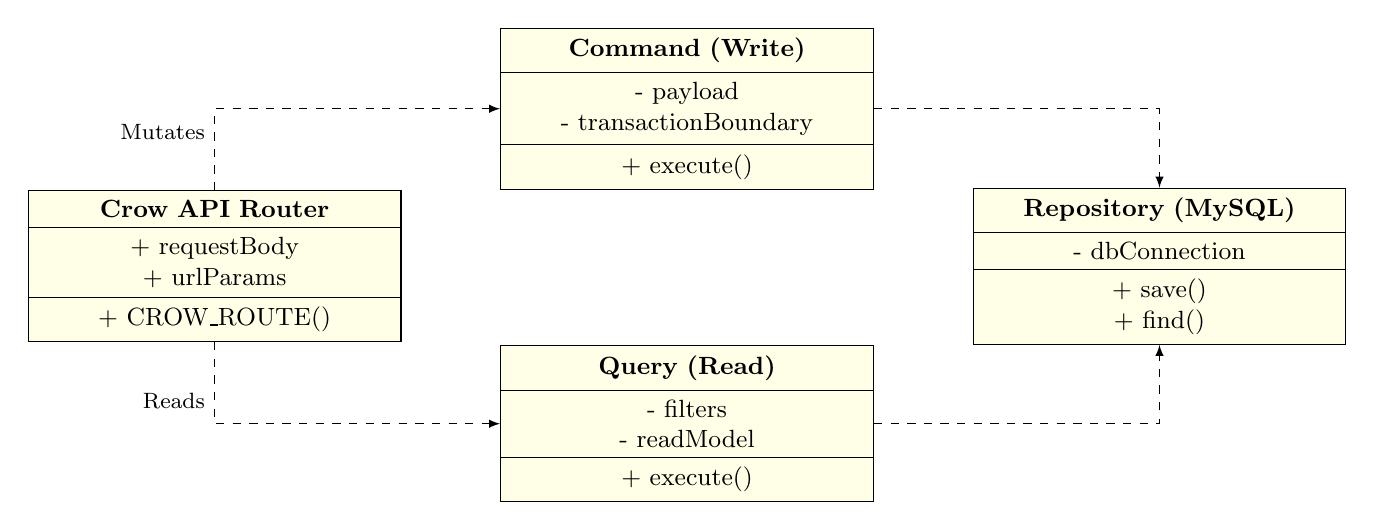
\begin{tikzpicture}[
    class/.style={draw, rectangle split, rectangle split parts=3, text centered, text width=4.5cm, font=\small, fill=yellow!10},
    line/.style={draw, -latex, dashed}
]

\node[class] (controller) at (0, 0) {
    \textbf{Crow API Router}
    \nodepart{second}
    + requestBody\\
    + urlParams
    \nodepart{third}
    + CROW\_ROUTE()
};

\node[class] (command) at (6, 2) {
    \textbf{Command (Write)}
    \nodepart{second}
    - payload\\
    - transactionBoundary
    \nodepart{third}
    + execute()
};

\node[class] (query) at (6, -2) {
    \textbf{Query (Read)}
    \nodepart{second}
    - filters\\
    - readModel
    \nodepart{third}
    + execute()
};

\node[class] (db) at (12, 0) {
    \textbf{Repository (MySQL)}
    \nodepart{second}
    - dbConnection
    \nodepart{third}
    + save()\\
    + find()
};

\draw[line] (controller) |- (command.west) node[near start, above left, font=\footnotesize] {Mutates};
\draw[line] (controller) |- (query.west) node[near start, below left, font=\footnotesize] {Reads};
\draw[line] (command.east) -| (db.north);
\draw[line] (query.east) -| (db.south);

\end{tikzpicture}
\caption{CQRS Architecture demonstrating separation of Commands and Queries.}
\end{figure}

\subsubsection{Database Schema (ER Diagram)}
\begin{figure}[h]
\centering
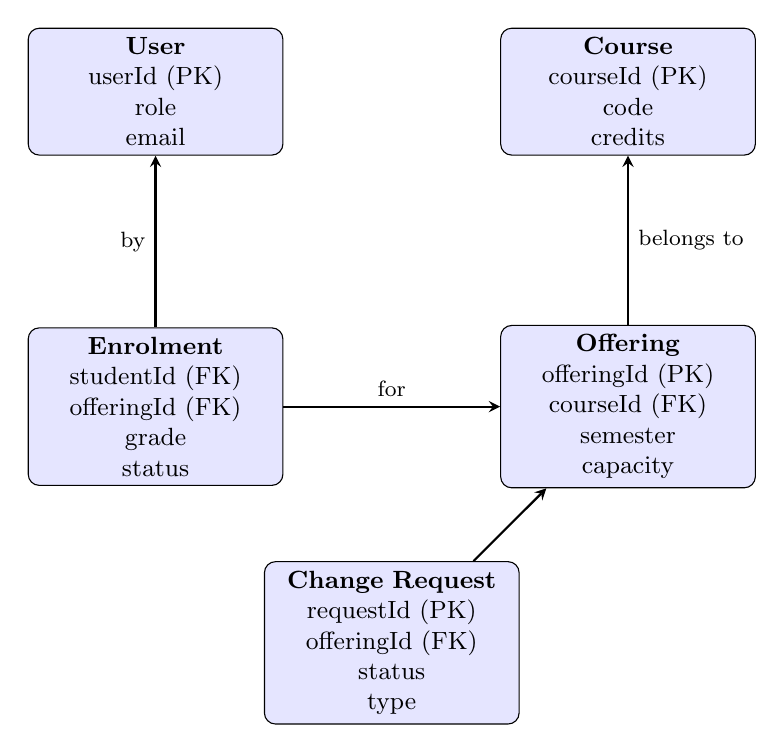
\begin{tikzpicture}[
    entity/.style={draw, rectangle, rounded corners, fill=blue!10, text centered, text width=3cm, font=\small},
    rel/.style={draw, diamond, aspect=2, text centered, font=\footnotesize, fill=green!10},
    line/.style={draw, thick, -stealth}
]

\node[entity] (user) at (0,0) {\textbf{User}\\userId (PK)\\role\\email};
\node[entity] (course) at (6,0) {\textbf{Course}\\courseId (PK)\\code\\credits};
\node[entity] (offering) at (6,-4) {\textbf{Offering}\\offeringId (PK)\\courseId (FK)\\semester\\capacity};
\node[entity] (enrolment) at (0,-4) {\textbf{Enrolment}\\studentId (FK)\\offeringId (FK)\\grade\\status};

\draw[line] (offering) -- node[right, font=\footnotesize]{belongs to} (course);
\draw[line] (enrolment) -- node[above, font=\footnotesize]{for} (offering);
\draw[line] (enrolment) -- node[left, font=\footnotesize]{by} (user);

\node[entity] (request) at (3,-7) {\textbf{Change Request}\\requestId (PK)\\offeringId (FK)\\status\\type};
\draw[line] (request) -- (offering);

\end{tikzpicture}
\caption{Simplified Entity-Relationship Diagram outlining the MySQL Database.}
\end{figure}

\subsubsection{Course Enrolment Workflow}
\begin{figure}[h]
\centering
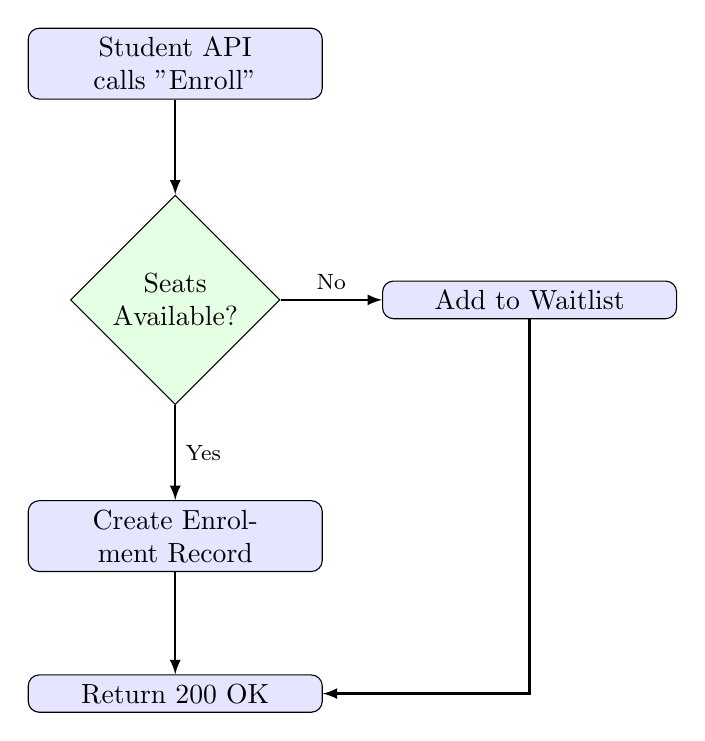
\begin{tikzpicture}[
    block/.style={rectangle, draw, fill=blue!10, text width=3.5cm, text centered, rounded corners, minimum height=1em},
    decision/.style={diamond, draw, fill=green!10, text width=2cm, text badly centered, node distance=2.5cm, inner sep=0pt},
    line/.style={draw, -latex, thick}
]

\node [block] (start) {Student API calls "Enroll"};
\node [decision, below of=start, node distance=3cm] (seats) {Seats Available?};
\node [block, right of=seats, node distance=4.5cm] (waitlist) {Add to Waitlist};
\node [block, below of=seats, node distance=3cm] (enroll) {Create Enrolment Record};
\node [block, below of=enroll, node distance=2cm] (success) {Return 200 OK};

\path [line] (start) -- (seats);
\path [line] (seats) -- node[above, font=\footnotesize] {No} (waitlist);
\path [line] (seats) -- node[right, font=\footnotesize] {Yes} (enroll);
\path [line] (enroll) -- (success);
\path [line] (waitlist) |- (success);

\end{tikzpicture}
\caption{Course Enrolment Workflow Logic.}
\end{figure}

\subsection{Software Design Principles}
\begin{itemize}
    \item \textbf{Single Responsibility:} A Command class like \texttt{EnrollStudentCommand} handles exactly one transaction. It delegates data fetching to the Repositories, adhering perfectly to SRP.
    \item \textbf{Open/Closed Principle:} New reports or features can be added by creating a new Query or Command class without modifying existing routing logic.
    \item \textbf{Dependency Inversion:} The API layer depends on abstract Command structures and Repository interfaces rather than concrete MySQL queries.
    \item \textbf{DRY:} Reusable utility functions for JSON parsing and error handling are centralized in \texttt{routes.cpp}.
\end{itemize}

\subsection{Implementation Notes}
The proof-of-concept is written in C++17 utilizing the Crow web framework and the MySQL C API. The frontend is a Vanilla HTML/CSS/JS Single Page Application served directly by Crow.
\begin{itemize}
    \item \textbf{Backend Code:} Located in \texttt{src/}. Divided into \texttt{business/cqrs} (Commands/Queries), \texttt{data/mysql} (Repositories), and \texttt{presentation/api} (Routes).
    \item \textbf{Frontend Code:} Located in \texttt{frontend/}. Contains \texttt{index.html}, \texttt{style.css}, and \texttt{app.js}.
    \item \textbf{Database:} Managed via SQL scripts in \texttt{database/mysql/}.
\end{itemize}
\textbf{How to run:}
\begin{enumerate}
    \item Initialize the MySQL database with \texttt{001\_schema.sql} and \texttt{002\_seed.sql}.
    \item Compile the C++ backend using \texttt{make}.
    \item Start the server via \texttt{make run}.
    \item Navigate to \texttt{http://localhost:8080} and login as \texttt{U-STU-001} (Student), \texttt{U-FAC-001} (Faculty), or \texttt{U-ADM-001} (Admin).
\end{enumerate}

\subsection{Interactive Web Application (SPA UI Layer)}
The team built a robust Single Page Application (SPA) utilizing HTML5, CSS3 Variables for dark-mode theming, and ES6 JavaScript to consume the C++ REST API seamlessly. The frontend routing is handled via hash-changes in \texttt{app.js}, dynamically rendering views based on user roles without page reloads. The UI successfully demonstrates live seat updates, dynamic waitlisting, and complex administrative reporting generated on-the-fly via the API.

\section{Assessment Criteria Cross-Reference}
\begin{table}[h]
\centering
\begin{tabular}{|p{5cm}|p{2cm}|p{5cm}|}
\hline
\textbf{Criterion} & \textbf{Weight} & \textbf{Addressed In} \\
\hline
Architectural Choice & 15\% & Sections 2.1–2.2 \\
Architectural Diagram & 15\% & Section 3.3.1 \\
Design Pattern Application & 40\% & Section 3.2, source code \\
Implementation \& Quality & 20\% & Section 3.5, source code \\
Documentation & 10\% & This report in full \\
\hline
\end{tabular}
\end{table}

\end{document}
